\section{Graded Assignment 1}\label{sec:graded_assignment_1}
The IMM-PDAF combines Interactive Multiple Models (IMM) with Probabilistic Data Association Filter (PDAF). Relevant theory can be found in \cite[p. 100-101, 120 - 122]{Edmund}. 

\subsection*{Results}
\subsubsection*{Simulated data set}
Tuning the full system for the simulated data required tuning of, in total, four systems. These were the Extended Kalman Filters, for the Constant Velocity and Constant Turn-rate modes, the IMM, and the IMM-PDAF. 

For the CV model, the measurement noise covariance parameter used was $4$, while the acceleration noise covariance parameter used was $\scinot{8}{-2}$. Similarly, the same measurement noise covariance parameter was used for the CT model, as the measurement noises should be similar. Furthermore, the acceleration noise covariance parameter used was $\scinot{5}{-3}$ and the turn-rate noise parameter used was $\scinot{3}{-4}$. Tuning these parameters would have some impact on the consistency, higher noise would lower the NEES, while lower noise increases the NEES, which is to be expected as we are essentially changing how much the filter should trust the measurements contra the estimates. From \cref{fig:ga_1_2_estimated_trajectory}, it can be seen that both models handle their trajectories well. 

The IMM was tuned using the transition matrix $\pi$, which was tuned as \cref{eq:ga_1_2_pi_matrix}. With the CV model as the first model and the CT model as the second, the argument is that if the IMM is in a given mode, it should most likely stay. Still, it may be beneficial to be more likely to change to, and stay as, the CT model. When observing the trajectory, see \cref{fig:ga_1_2_estimated_trajectory}, it seems to primarily use the CV model, and then increasing the transition probability for changing to the CT model would speed up this transition. The probabilities over time can then be seen from \cref{fig:ga_1_2_probabilities}.

\begin{equation}
    \label{eq:ga_1_2_pi_matrix}
    \pi = \begin{bmatrix}
        0.92 & 0.05 \\
        0.08 & 0.95
    \end{bmatrix}
\end{equation}

\begin{figure}[ht]
    \begin{subfigure}[h]{0.4\textwidth}
        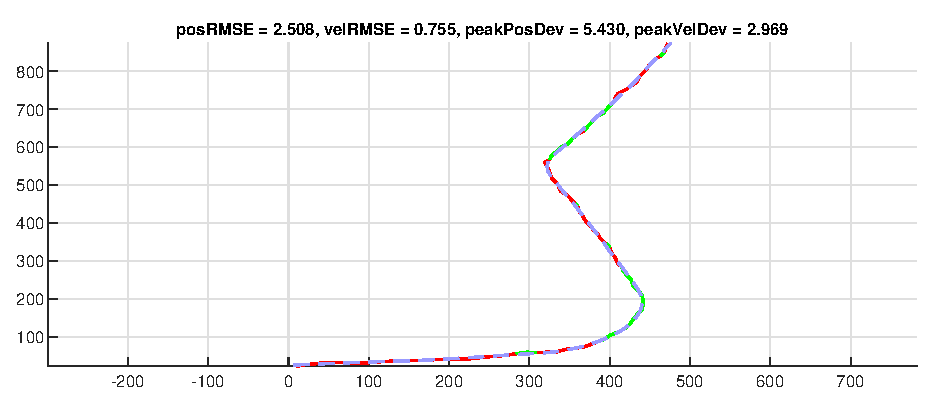
\includegraphics[width=\textwidth]{figures/ga_1/2_estimated_trajectory}
        \caption{Trajectory for simulated data}
        \label{fig:ga_1_2_estimated_trajectory}
    \end{subfigure}%
    ~
    \begin{subfigure}[h]{0.4\textwidth}
        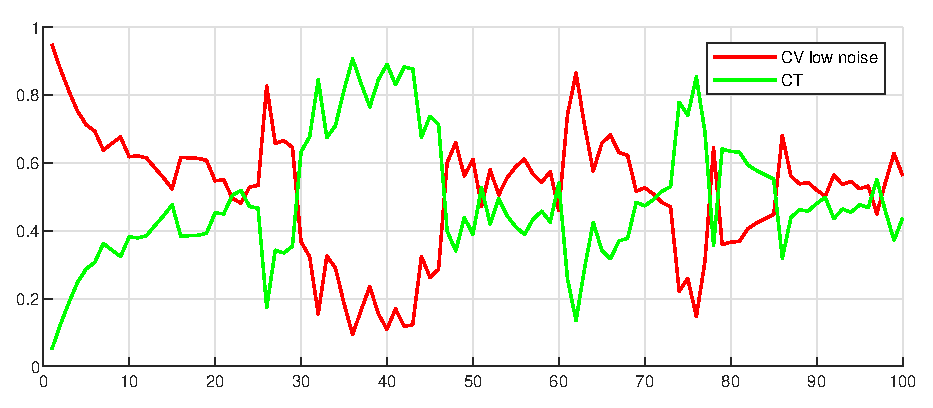
\includegraphics[width=\textwidth]{figures/ga_1/2_probs}
        \caption{Probabilities simulated data}
        \label{fig:ga_1_2_probabilities}
    \end{subfigure}
    \caption{The same colour code was utilised for visualising the active modes in the trajectory as the probability. For the trajectory, ground truth is represented as a dashed line. }
    \label{fig:ga_1_2_traj_and_probs} 
\end{figure}

Finally, for the IMM-PDAF, the clutter rate $\lambda$, detection probability $P_D$ and the validation gate were tuned. The clutter rate was tuned to $\lambda = \scinot{1}{-4}$, and as there were very few false alarms, this could be chosen as a low value. Furthermore, as the only place the clutter rate is used in the IMM-PDAF is to scale the probability of no detection, there was really no use further decreasing $\lambda$, as it already would put the association likelihood ratio for no detection very low. The detection probability is tuned to be rather high, with $P_D = 0.95$, as it is expected that there is a good chance of detection for this data set. A validation gate size of $5^2$ seemed also to give decent results. Increasing it would generally not make the tracker worse overall, but would increase the magnitude of certain errors, which would then spike. Decreasing it would of course make it more difficult for any measurements to be gated, such that this value seemed to be the best compromise between gating all and no measurements. The resulting consistency plot can be seen as \cref{fig:ga_1_2_NEES}, and the average NEES were for position $1.9248$, for velocity $1.1427$ and overall $3.0887$. The errors seem generally ok, and limited in amplitude, as seen from \cref{fig:ga_1_2_error}. 

\begin{figure}[ht]
	\begin{subfigure}[h]{0.4\textwidth}
		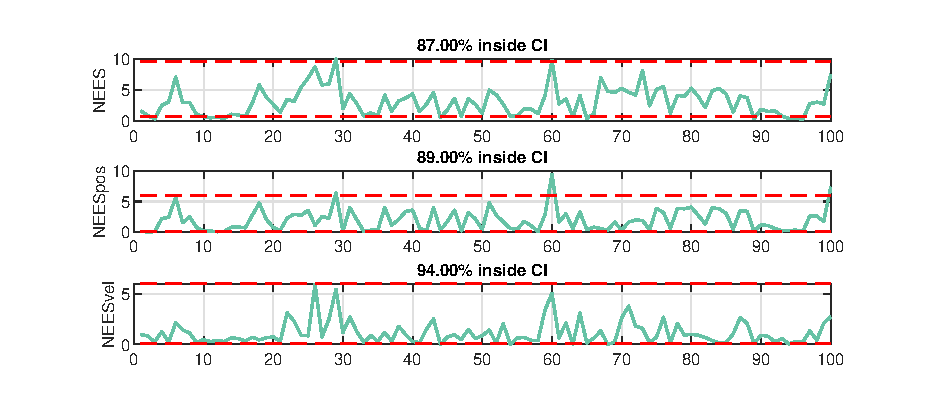
\includegraphics[width=\textwidth]{figures/ga_1/2_NEES}
		\caption{NEES for simulated data}
		\label{fig:ga_1_2_NEES}
    \end{subfigure}% 
    ~
    \begin{subfigure}[h]{0.4\textwidth}
        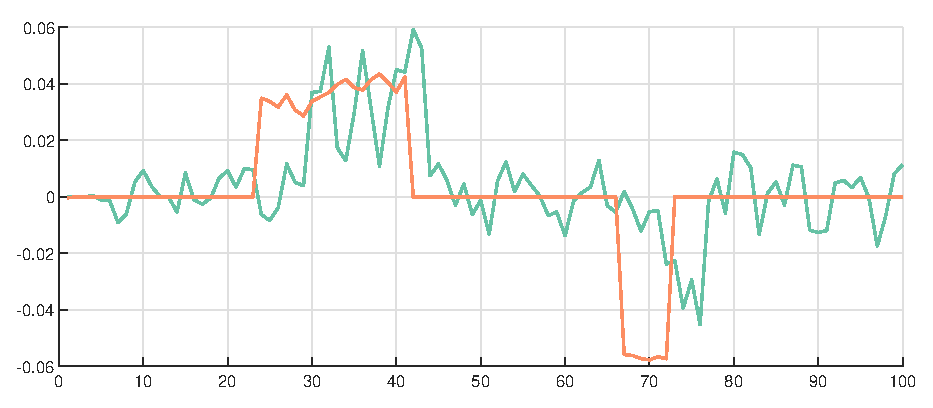
\includegraphics[width=\textwidth]{figures/ga_1/2_error}
        \caption{Errors for simulated data}
        \label{fig:ga_1_2_error}
    \end{subfigure}
    \caption{The NEES and errors from the simulated data. }
    \label{fig:ga_1_2_NEES_and_error} 
\end{figure}

\subsubsection*{Joyride data set}
Initially, the IMM-PDAF for the Joyride data set was tuned similarly to the tracker for the simulated data set, and especially for the low noise CV model and the CT model, similar values were used. Furthermore, it should be noted that the Joyride data set also was noisier, such that more lenient tuning was necessary. For this data set, a high noise CV model was also included, which could \textit{take over} if both the low noise CV model and the CT model were uncertain. Otherwise, the overall structure of the tracker is the same as for the simulated data set. 

The measurement noise covariance parameter was again the same for the CT and two CV models, and was set to $25^2$. Though this seemed rather higher than necessary, however lowering it would especially push the positional NEES too high. Similar responses were generated from tuning the acceleration noise covariance parameters and turn-rate noise covariance parameter for the different models. Then, for the low noise CV model, the acceleration noise covariance parameter was tuned to $0.5$, for the high noise CV model, the acceleration noise covariance parameter was tuned to $20$ and for the CT model, the acceleration noise covariance parameter was tuned to $\scinot{1}{-4}$ and the turn-rate noise covariance parameter was tuned to $\scinot{2}{-4}$. Similarly to the results from the simulated data, these models handle their trajectories well, as can be seen from \cref{fig:ga_1_joyride_estimated_trajectory}. 

As for the IMM used in the simulated data set, the transition matrix $\pi$ was tuned to prefer to stay in the CT model, so that the tracker should prefer to continue a turn if it was already turning. Since the high noise CV model was included primarily to handle high noise areas where it could be unambiguous whether to use the low noise CV or CT model, this transition probability was set lower than the others, as those should be preferred. From observing the track and measurements, there also seemed to be unambiguous which of the other modes each should transition to, and as such these transitions were set to be equally likely, see \cref{eq:ga_1_joyride_pi_matrix}. The resulting changes to the probabilities can be seen from \cref{fig:ga_1_joyride_probabilities}. 

\begin{equation}
    \label{eq:ga_1_joyride_pi_matrix}
    \pi = \begin{bmatrix}
        0.900 & 0.025 & 0.075 \\
        0.050 & 0.950 & 0.075 \\
        0.050 & 0.025 & 0.850 
    \end{bmatrix}
\end{equation}

\begin{figure}[ht]
    \begin{subfigure}[h]{0.4\textwidth}
        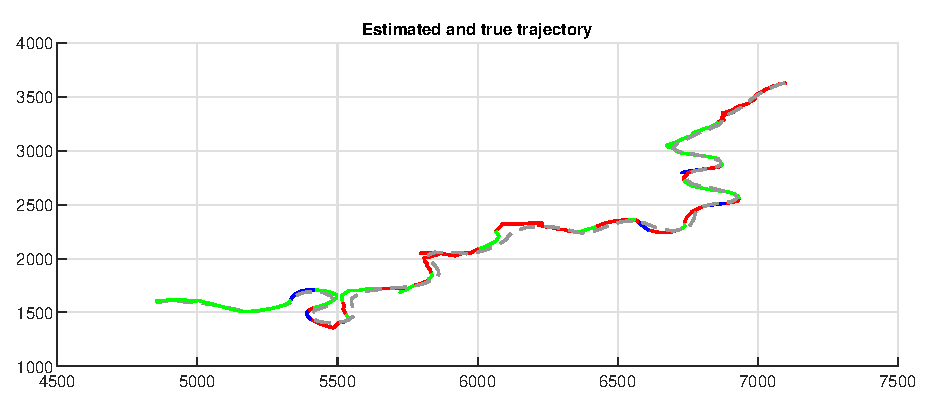
\includegraphics[width=\textwidth]{figures/ga_1/joyride_estimated_trajectory}
        \caption{Trajectory for joyride data}
        \label{fig:ga_1_joyride_estimated_trajectory}
    \end{subfigure}%
    ~
    \begin{subfigure}[h]{0.4\textwidth}
        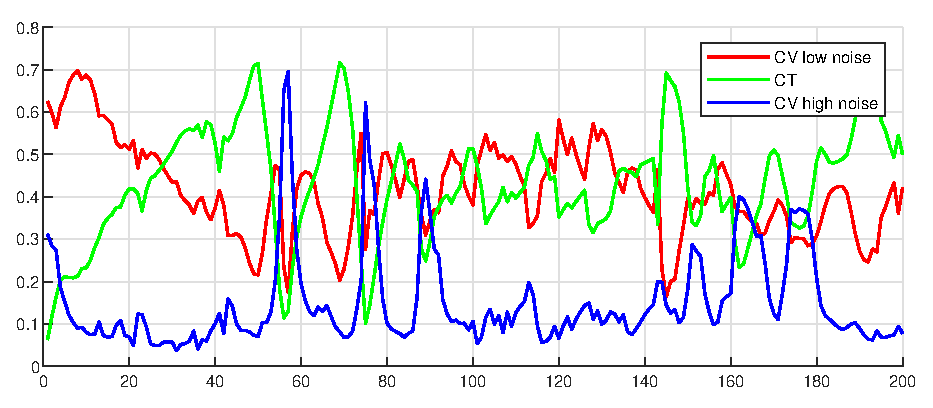
\includegraphics[width=\textwidth]{figures/ga_1/joyride_probs}
        \caption{Probabilities joyride data}
        \label{fig:ga_1_joyride_probabilities}
    \end{subfigure}
    \caption{The same colour code was utilised for visualising the active modes in the trajectory as the probability. For the trajectory, ground truth is represented as a dashed line. }
    \label{fig:ga_1_joyride_traj_and_probs} 
\end{figure}

The IMM-PDAF was tuned to have a lower clutter rate and higher detection probability than for the simulated data, while keeping the gate size. The clutter rate was tuned to be $\lambda = \scinot{5}{-5}$. Higher values would inevitably make the tracker loose track and converge to one mode, rendering the tracker useless. As the clutter rate affects the likelihood ratio for no detection, a higher clutter rate implies a higher likelihood compared to a lower clutter rate, and a higher value would be given to the association probability for no detection. The detection probability was tuned to $P_D = 0.97$, which is a rather high value. It was possible to reduce $P_D$ and, specifically, improve the percentage where the NEES is inside CI, but at a cost of the NEES for the velocity, and a higher $P_D$ was chosen so that the NEESes would be more similar. 

The resulting consistency plot can be seen \cref{fig:ga_1_joyride_NEES}, and the average NEESes were found as $1.6653$ for position, $1.3966$ for velocity and $3.4346$ overall. Both the plots and the averages tend to be closer to the lower bound of the confidence interval, though as can be noted, there were certain spikes in the plot. These were difficult to handle as they seemed to originate from especially bad measurements, and a compromise was made where the consistency would tend to be low, in exchange for limiting the spikes. The errors also seemed to be acceptable, see \cref{fig:ga_1_joyride_error}. 

\begin{figure}[ht]
	\begin{subfigure}[h]{0.4\textwidth}
		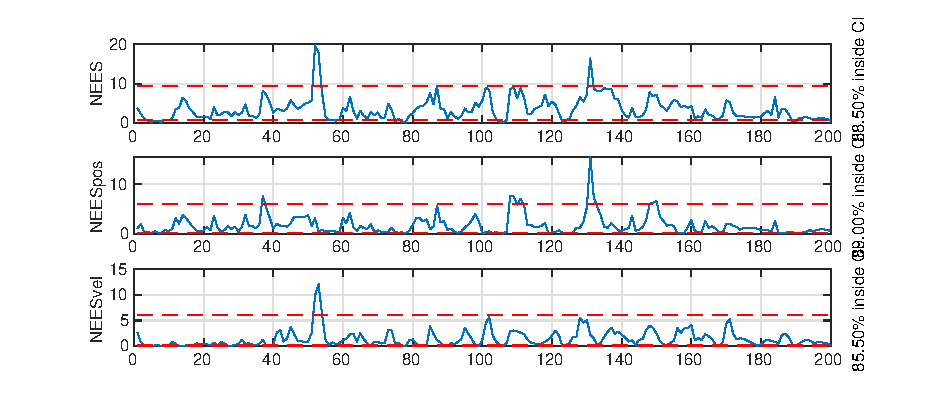
\includegraphics[width=\textwidth]{figures/ga_1/joyride_NEES}
		\caption{NEES for joyride data}
		\label{fig:ga_1_joyride_NEES}
    \end{subfigure}% 
    ~
    \begin{subfigure}[h]{0.4\textwidth}
        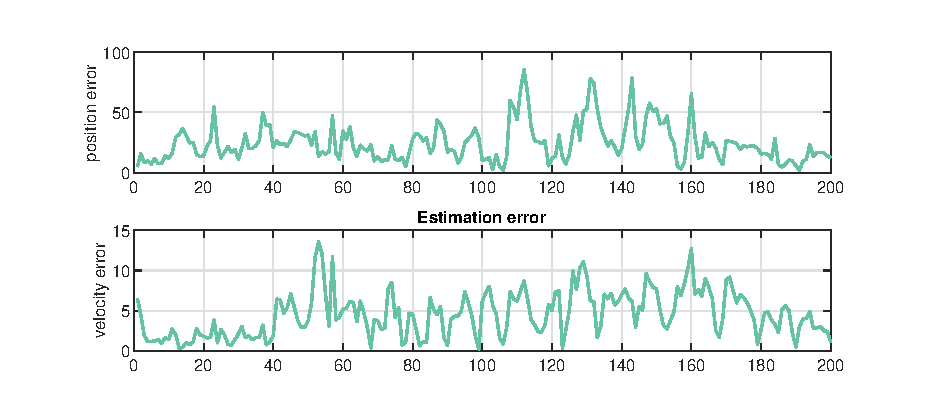
\includegraphics[width=\textwidth]{figures/ga_1/joyride_error}
        \caption{Errors for joyride data}
        \label{fig:ga_1_joyride_error}
    \end{subfigure}
    \caption{The NEES and errors from the joyride data. }
    \label{fig:ga_1_joyride_NEES_and_error} 
\end{figure}

% stepsWithClose =
%    136
% meanMeasError =
%     3.6865
%    -7.2491
% covMeasError =
%   119.3970   14.9059
%    14.9059  116.2221
% stds =
%    10.9269
%    10.7806
% covEllSize =
%    10.1400
%    11.5239
% meanMinMeasDists =
%   300.0264
% meanNumberOfCloseMeasurements =
%     0.6800
% CI2K =
%     1.7324    2.2865
% ANEESpos =
%     1.6653
% ANEESvel =
%     1.3966
% CI4K =
%     3.6176    4.4014
% ANEES =
%     3.4346

% note that q lower for CT? 

% parameters 

% In the report you should do a bit more analysis of what happens with different parameters settings, and base your choice on relevant plots and numbers. To achieve a full score we also want to see at least some minor reflections on the algorithm and the approximations it does in light of your results. 
% We want to see an analysis of what happens and why with some different parameter/model settings, and base your choice of model and parameters on relevant plots and numbers. To achieve a full score we also want to see at least some minor reflections on the algorithm and the approximations it does, in light of your results. Relating results in this tasks or assignments to the previous task can give additional points. 

% \begin{figure}[ht]
% 	\begin{subfigure}[h]{0.4\textwidth}
% 		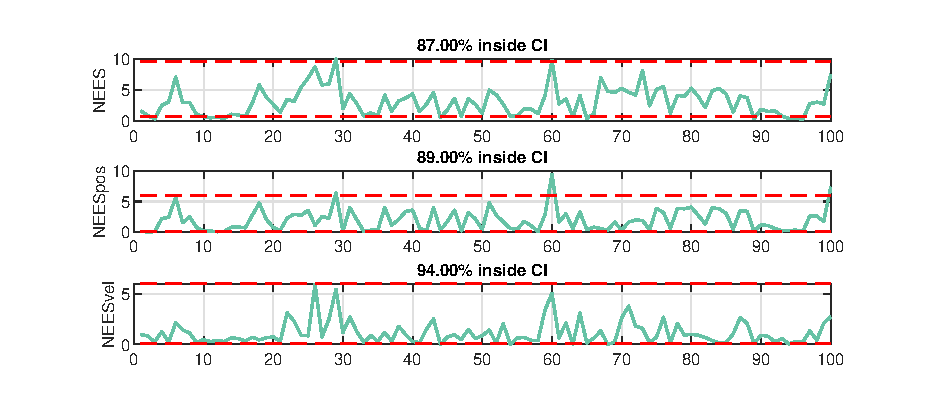
\includegraphics[width=\textwidth]{figures/ga_1/2_NEES}
% 		\caption{NEES for simulated data}
% 		\label{fig:ga_1_2_NEES}
%     \end{subfigure}%
%     ~
% 	\begin{subfigure}[h]{0.4\textwidth}
% 		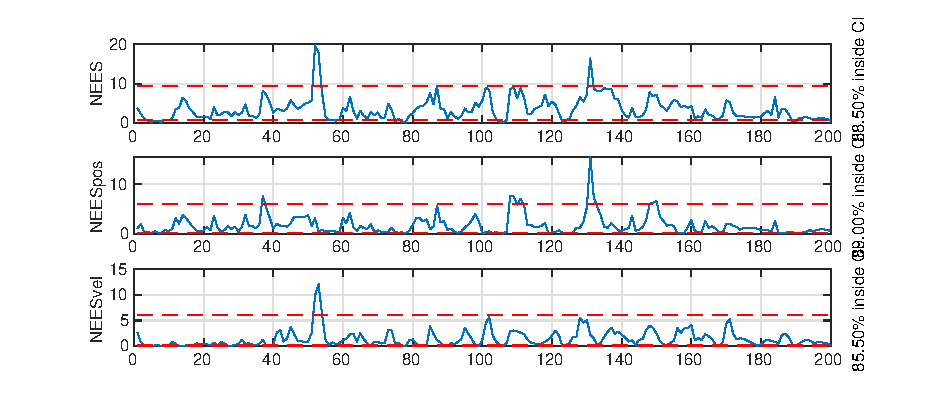
\includegraphics[width=\textwidth]{figures/ga_1/joyride_NEES}
% 		\caption{NEES for Joyride}
% 		\label{fig:ga_1_joyride_NEES}
% 	\end{subfigure}
%         \\
%     \begin{subfigure}[h]{0.4\textwidth}
%         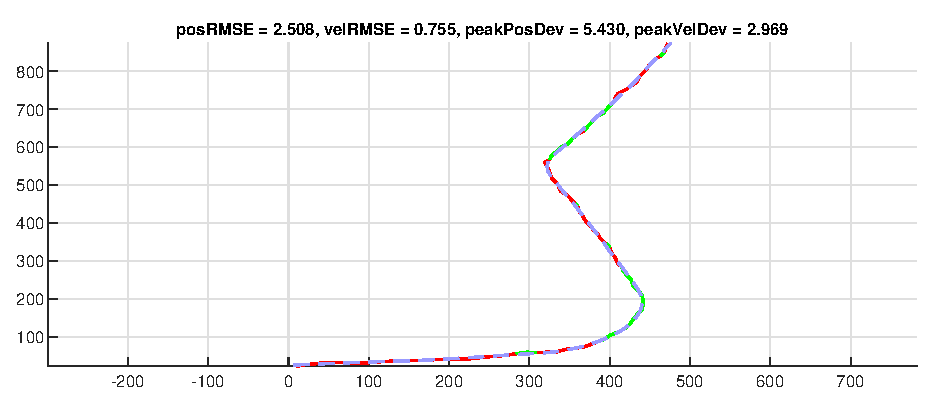
\includegraphics[width=\textwidth]{figures/ga_1/2_estimated_trajectory}
%         \caption{Trajectory for simulated data}
%         \label{fig:ga_1_2_estimated_trajectory}
%     \end{subfigure}%
%     ~
%     \begin{subfigure}[h]{0.4\textwidth}
%         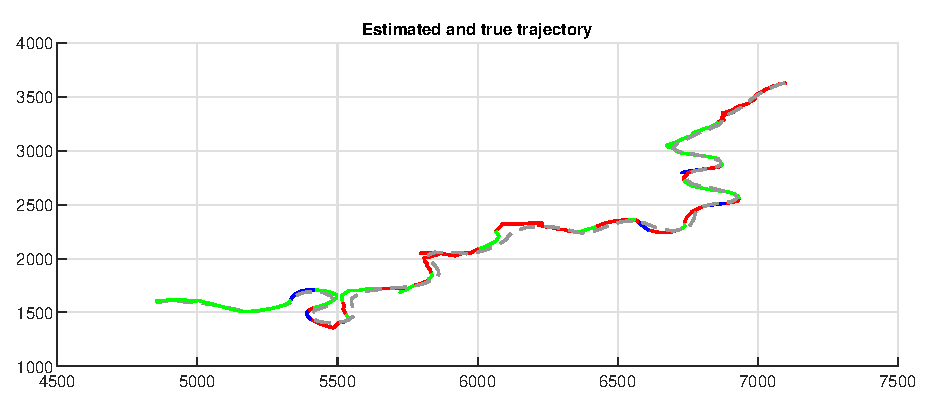
\includegraphics[width=\textwidth]{figures/ga_1/joyride_estimated_trajectory}
%         \caption{Trajectory for Joyride}
%         \label{fig:ga_1_joyride_estimated_trajectory}
%     \end{subfigure}
%         \\
%     \begin{subfigure}[h]{0.4\textwidth}
%         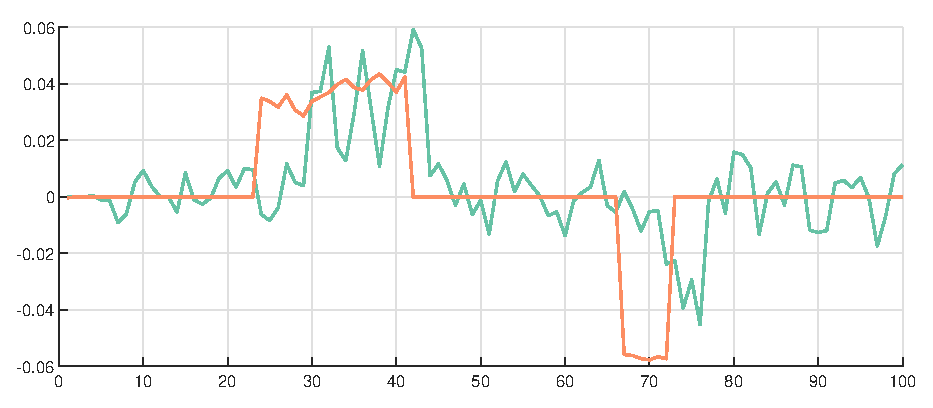
\includegraphics[width=\textwidth]{figures/ga_1/2_error}
%         \caption{Errors for simulated data}
%         \label{fig:ga_1_2_error}
%     \end{subfigure}%
%     ~
%     \begin{subfigure}[h]{0.4\textwidth}
%         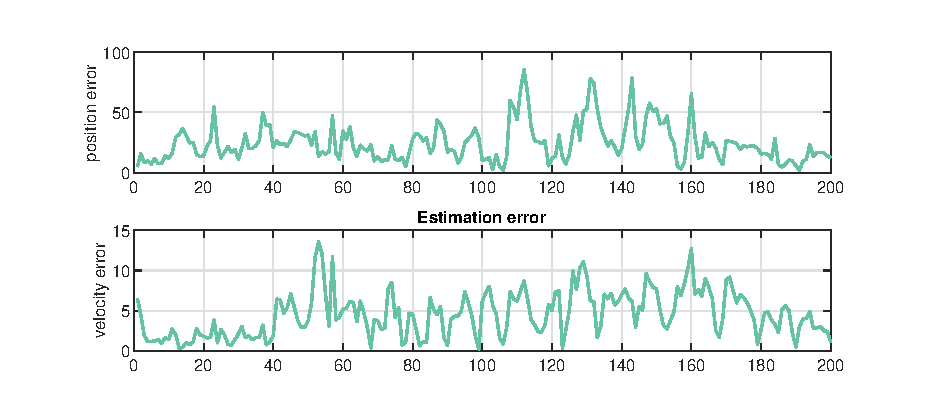
\includegraphics[width=\textwidth]{figures/ga_1/joyride_error}
%         \caption{Errors for Joyride}
%         \label{fig:ga_1_joyride_error}
%     \end{subfigure}
%         \\
%     \begin{subfigure}[h]{0.4\textwidth}
%         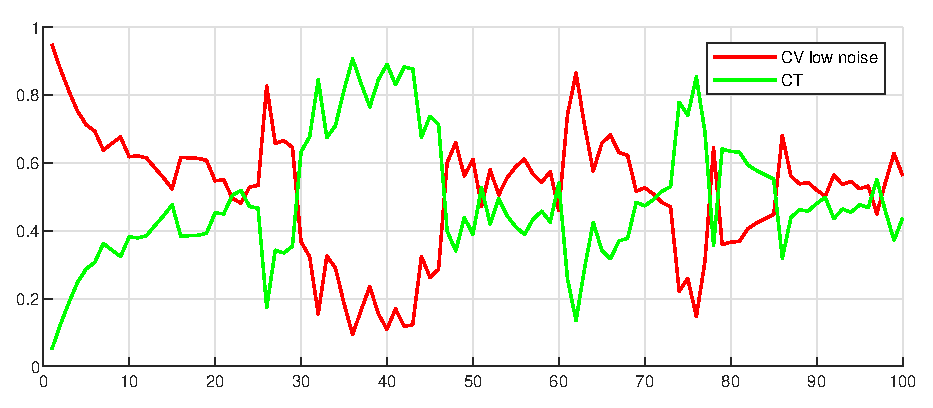
\includegraphics[width=\textwidth]{figures/ga_1/2_probs}
%         \caption{Probabilities simulated data}
%         \label{fig:ga_1_2_probabilities}
%     \end{subfigure}%
%     ~
%     \begin{subfigure}[h]{0.4\textwidth}
%         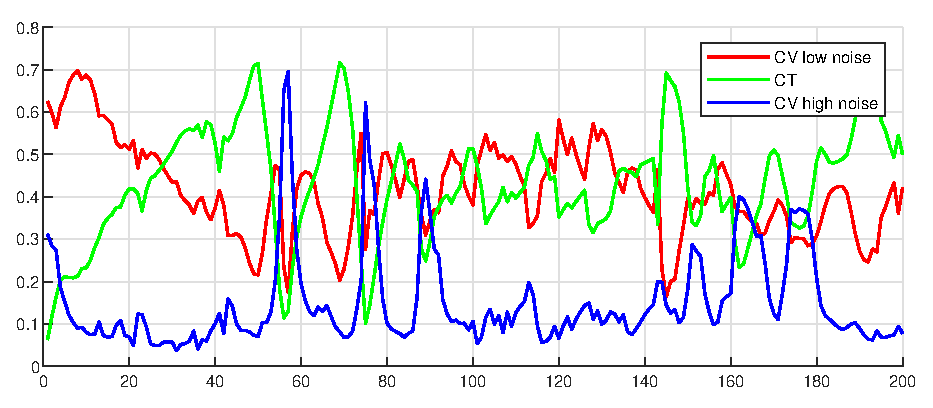
\includegraphics[width=\textwidth]{figures/ga_1/joyride_probs}
%         \caption{Probabilities for Joyride}
%         \label{fig:ga_1_joyride_probabilities}
%     \end{subfigure}
%     \caption{The same colour code was utilised for visualising the active modes in the trajectories as the probabilities. For the trajectories, ground truth is represented as a dashed line. }
%     \label{fig:ga_1} 
% \end{figure}

\subsection*{Assumptions}
The IMM-PDAF works under the single-target assumptions, as seen from \cite[p. 105]{Edmund}, which all seem reasonable considering both the simulated and real data sets. In the simulated data set, there is initially good reason to suspect that these assumptions were considered when the data set was generated, and it may therefore be more interesting to consider the real data set. There are a smaller number of measurements for each time step than there seemed to be for the simulated data set, and therefore, it may seem like the job of the tracker for this data set is, primarily, to consider whether there is a detection or not. In certain cases, the measurements are also pretty far away from each other and the track, which could also make it easier for the tracker. Since it is likely that several raw measurements may originate from the sensor, like a RADAR, it is common to apply some form of clustering to reduce the measurements from the target to one single measurement. Depending on the method for clustering, this is very likely to make the tracker work, and it is computationally a good idea to use the single target assumption, though this clustering may also cluster bad measurements as well, which may make the tracking more difficult. This was not further explored here, as there doesn't seem to be a need for it. 

% IMM-PDAF
There are certain simplifications done in this algorithm to make it more viable, and as mentioned above, assuming that only one measurement may originate from the target allows for a more computationally efficient algorithm. Additionally, as the associations (and modes) are seen as mixtures, then as to not end up with an extremely large number of values, the mixtures can be reduced by moment matching. This also makes the tracker a more computationally efficient algorithm, and keeps the memory usage manageable. 

% gate
    % at least one is gated
Gating of the measurements, is done, for each measurement, by checking the NISes for all modes given this measurement. If a measurement is gated for one mode, it is gated for all modes. This assumption seems to be good, as it then seems like at least one of the models can \textit{accept} this measurement. There may still be cases where a stricter gating rule could have been considered, like only applying the measurements to the specific modes with NISes within the gate size. For these data sets however, there haven't been any specific cases where this assumption has caused problems. 

% IMM
Certain simplifications were also made to make the code easier to implement, which probably slows the tracker slightly down, as when calculating the log-likelihood ratios, the \textit{update}-method from the IMM was utilised, and most of the results were discarded. If there was a need to save a small amount of time, or reduce the number of operations done, there are some places in the code where one could save time. This could be necessary if there was a need to run the tracker online. 

% EKF
Using the EKF, with the CV and CT models, is also a simplification, especially for the joyride data set. For the simulated data set, these models were probably used to generate the data set. It should therefore be possible to get very good result using these models, as seen from \cref{fig:ga_1_2_estimated_trajectory}. The joyride data set, however, is different, as there is not \textit{really} an underlying model which generated this data set. Still, by using several simpler models, including a high-noise mode for robustness, decent tracking was achieved for the joyride data set as well, as can be seen from \cref{fig:ga_1_joyride_estimated_trajectory}. 

% task 2 and 3
    % NEES with confidence bounds
        % total
        % position
        % velocity
    % estimation error (Euclidian distance)
        % position 
        % velocity
    % averaged NEESes 
    % number of times the NEESes fall within the confidence region
    % position and velocity RMSE (mean taken over time)

% parameters based on this
% other plots




% For task 2 and 3, we want to see a plot of the total, position and velocity NEES along with your chosen confidence bounds for these, and estimation error (Euclidian distance) in position and velocity for the tracker run with your chosen parameters. 
% In addition we want the numbers of the averaged NEESes along with their confidence bounds, the number of times the NEESes fall within the confidence regions and the positional and velocity RMSE (mean taken over time). 
% We then expect you to base your choice of parameters on these values, and compare to other sets of parameters. 
% To show plots of other parameter settings is up to you. 